How does Thread id work? implicitly passed to each thread??

do not use figure, but ref to mortens and then show how to use it!
\autoref{fig:memory-hierarchy}

\begin{figure}[ht]
	\centering
	\fbox{
		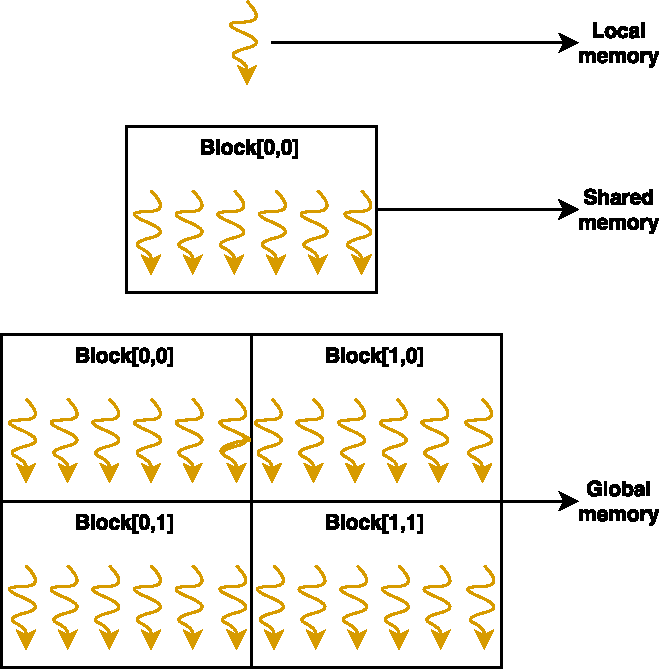
\includegraphics[width=0.6\textwidth]{figs/programming-model/memory-hierarchy.pdf}
	}
	\caption{Memory hierarchy}
	\label{fig:memory-hierarchy}
\end{figure}


copy to device etc
d\_ pointers etc
shared memory
global memory etc and how to do it

